\section{Anfängerfehler}

\begin{figure}[!b]
 \begin{center}
  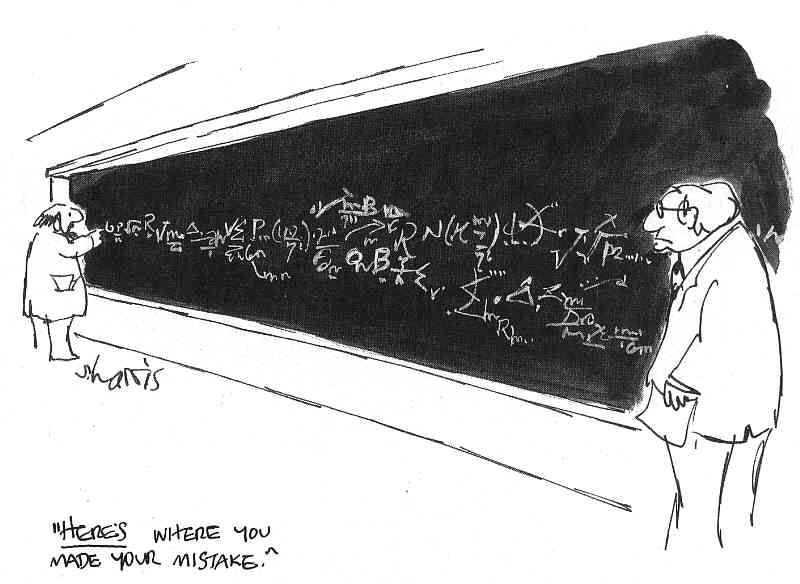
\includegraphics[height=6.5 cm]{bilder/mistake.jpg}
 \end{center}
\end{figure}

Das Wichtigste in der Anfängerzeit ist eigentlich: "`Büffeln, büffeln und noch mal büffeln``.\\
Besonders in Mathe und Theo--Physik werdet ihr bald zu der
Erkenntnis kommen, dass das, was die Professoren oft als so
"`trivial`` bezeichnen, in den Übungszetteln doch nicht so einfach ist.
Man kann natürlich die Zettel beim jeweiligen Matheass abschreiben.
Aber leider hat das keinen Sinn, da ihr den Stoff spätestens in der nächsten Modulprüfung brauchen werdet.\\
Und wie immer gilt auch hier die Regel:\\
"`\textbf{Ein selbst gemachter Fehler ist besser als eine abgeschriebene Musterlösung}.``\\
Naja, so viel dazu.
%
Ein anderer Punkt sind die Tutorien.
Es kann passieren, dass ihr euch einen Tutor aussucht, der vielleicht ganz
nett aussieht (und es höchst wahrscheinlich auch ist), dessen Stil
euch aber ganz und gar nicht liegt, weil er vielleicht die
Vektorpfeile unter die Variablen setzt oder so.
Vielleicht macht ihr ja ein Doppelstudium und zur Zeit eures Theoretikums habt ihr gerade
eine Vorlesung über Morphologie und Syntax afrikanischer Sprachen.\\
Das ist aber kein Problem, da ihr die Tutorien einfach wechseln könnt.
Besonders einfach geht das in der theoretischen Physik, da es dort unzählige Theoretika gibt.\\
%
Die wichtigste Regel lautet aber: "`Lernt in Gruppen!{}``.
Am meisten kann man lernen, wenn man die Themen der Vorlesung und die Übungszettel durchdiskutiert.
Des Weiteren findet man in einer Gruppe immer einen, der ein ganz bestimmtes Problem kennt.\\
Fragt! Fragt!! Und nochmals: Fragt!!!
Fragt Leute aus eurem Semester, fragt Leute aus den höheren Semestern und fragt die Professoren.
Gerade Professoren sind meistens begeistert über gute Fragen und stehen nach der Vorlesung
meistens sowieso noch an der Tafel herum.\\
%
Zu guter Letzt ist noch zu sagen: Lasst euch nicht hängen und gebt nicht auf.
Denn manchmal muss man sich ein bisschen anstrengen, um über den Berg zu kommen!

\von{Fritz}
